% Options for packages loaded elsewhere
\PassOptionsToPackage{unicode}{hyperref}
\PassOptionsToPackage{hyphens}{url}
%
\documentclass[
  ignorenonframetext,
]{beamer}
\usepackage{pgfpages}
\setbeamertemplate{caption}[numbered]
\setbeamertemplate{caption label separator}{: }
\setbeamercolor{caption name}{fg=normal text.fg}
\beamertemplatenavigationsymbolsempty
% Prevent slide breaks in the middle of a paragraph
\widowpenalties 1 10000
\raggedbottom
\setbeamertemplate{part page}{
  \centering
  \begin{beamercolorbox}[sep=16pt,center]{part title}
    \usebeamerfont{part title}\insertpart\par
  \end{beamercolorbox}
}
\setbeamertemplate{section page}{
  \centering
  \begin{beamercolorbox}[sep=12pt,center]{part title}
    \usebeamerfont{section title}\insertsection\par
  \end{beamercolorbox}
}
\setbeamertemplate{subsection page}{
  \centering
  \begin{beamercolorbox}[sep=8pt,center]{part title}
    \usebeamerfont{subsection title}\insertsubsection\par
  \end{beamercolorbox}
}
\AtBeginPart{
  \frame{\partpage}
}
\AtBeginSection{
  \ifbibliography
  \else
    \frame{\sectionpage}
  \fi
}
\AtBeginSubsection{
  \frame{\subsectionpage}
}
\usepackage{lmodern}
\usepackage{amssymb,amsmath}
\usepackage{ifxetex,ifluatex}
\ifnum 0\ifxetex 1\fi\ifluatex 1\fi=0 % if pdftex
  \usepackage[T1]{fontenc}
  \usepackage[utf8]{inputenc}
  \usepackage{textcomp} % provide euro and other symbols
\else % if luatex or xetex
  \usepackage{unicode-math}
  \defaultfontfeatures{Scale=MatchLowercase}
  \defaultfontfeatures[\rmfamily]{Ligatures=TeX,Scale=1}
\fi
% Use upquote if available, for straight quotes in verbatim environments
\IfFileExists{upquote.sty}{\usepackage{upquote}}{}
\IfFileExists{microtype.sty}{% use microtype if available
  \usepackage[]{microtype}
  \UseMicrotypeSet[protrusion]{basicmath} % disable protrusion for tt fonts
}{}
\makeatletter
\@ifundefined{KOMAClassName}{% if non-KOMA class
  \IfFileExists{parskip.sty}{%
    \usepackage{parskip}
  }{% else
    \setlength{\parindent}{0pt}
    \setlength{\parskip}{6pt plus 2pt minus 1pt}}
}{% if KOMA class
  \KOMAoptions{parskip=half}}
\makeatother
\usepackage{xcolor}
\IfFileExists{xurl.sty}{\usepackage{xurl}}{} % add URL line breaks if available
\IfFileExists{bookmark.sty}{\usepackage{bookmark}}{\usepackage{hyperref}}
\hypersetup{
  pdftitle={Final Presentation},
  pdfauthor={Collin Brehmer, Molly Hischke, Kyle Hancock, Nikki Johnson},
  hidelinks,
  pdfcreator={LaTeX via pandoc}}
\urlstyle{same} % disable monospaced font for URLs
\newif\ifbibliography
\usepackage{color}
\usepackage{fancyvrb}
\newcommand{\VerbBar}{|}
\newcommand{\VERB}{\Verb[commandchars=\\\{\}]}
\DefineVerbatimEnvironment{Highlighting}{Verbatim}{commandchars=\\\{\}}
% Add ',fontsize=\small' for more characters per line
\usepackage{framed}
\definecolor{shadecolor}{RGB}{248,248,248}
\newenvironment{Shaded}{\begin{snugshade}}{\end{snugshade}}
\newcommand{\AlertTok}[1]{\textcolor[rgb]{0.94,0.16,0.16}{#1}}
\newcommand{\AnnotationTok}[1]{\textcolor[rgb]{0.56,0.35,0.01}{\textbf{\textit{#1}}}}
\newcommand{\AttributeTok}[1]{\textcolor[rgb]{0.77,0.63,0.00}{#1}}
\newcommand{\BaseNTok}[1]{\textcolor[rgb]{0.00,0.00,0.81}{#1}}
\newcommand{\BuiltInTok}[1]{#1}
\newcommand{\CharTok}[1]{\textcolor[rgb]{0.31,0.60,0.02}{#1}}
\newcommand{\CommentTok}[1]{\textcolor[rgb]{0.56,0.35,0.01}{\textit{#1}}}
\newcommand{\CommentVarTok}[1]{\textcolor[rgb]{0.56,0.35,0.01}{\textbf{\textit{#1}}}}
\newcommand{\ConstantTok}[1]{\textcolor[rgb]{0.00,0.00,0.00}{#1}}
\newcommand{\ControlFlowTok}[1]{\textcolor[rgb]{0.13,0.29,0.53}{\textbf{#1}}}
\newcommand{\DataTypeTok}[1]{\textcolor[rgb]{0.13,0.29,0.53}{#1}}
\newcommand{\DecValTok}[1]{\textcolor[rgb]{0.00,0.00,0.81}{#1}}
\newcommand{\DocumentationTok}[1]{\textcolor[rgb]{0.56,0.35,0.01}{\textbf{\textit{#1}}}}
\newcommand{\ErrorTok}[1]{\textcolor[rgb]{0.64,0.00,0.00}{\textbf{#1}}}
\newcommand{\ExtensionTok}[1]{#1}
\newcommand{\FloatTok}[1]{\textcolor[rgb]{0.00,0.00,0.81}{#1}}
\newcommand{\FunctionTok}[1]{\textcolor[rgb]{0.00,0.00,0.00}{#1}}
\newcommand{\ImportTok}[1]{#1}
\newcommand{\InformationTok}[1]{\textcolor[rgb]{0.56,0.35,0.01}{\textbf{\textit{#1}}}}
\newcommand{\KeywordTok}[1]{\textcolor[rgb]{0.13,0.29,0.53}{\textbf{#1}}}
\newcommand{\NormalTok}[1]{#1}
\newcommand{\OperatorTok}[1]{\textcolor[rgb]{0.81,0.36,0.00}{\textbf{#1}}}
\newcommand{\OtherTok}[1]{\textcolor[rgb]{0.56,0.35,0.01}{#1}}
\newcommand{\PreprocessorTok}[1]{\textcolor[rgb]{0.56,0.35,0.01}{\textit{#1}}}
\newcommand{\RegionMarkerTok}[1]{#1}
\newcommand{\SpecialCharTok}[1]{\textcolor[rgb]{0.00,0.00,0.00}{#1}}
\newcommand{\SpecialStringTok}[1]{\textcolor[rgb]{0.31,0.60,0.02}{#1}}
\newcommand{\StringTok}[1]{\textcolor[rgb]{0.31,0.60,0.02}{#1}}
\newcommand{\VariableTok}[1]{\textcolor[rgb]{0.00,0.00,0.00}{#1}}
\newcommand{\VerbatimStringTok}[1]{\textcolor[rgb]{0.31,0.60,0.02}{#1}}
\newcommand{\WarningTok}[1]{\textcolor[rgb]{0.56,0.35,0.01}{\textbf{\textit{#1}}}}
\usepackage{graphicx,grffile}
\makeatletter
\def\maxwidth{\ifdim\Gin@nat@width>\linewidth\linewidth\else\Gin@nat@width\fi}
\def\maxheight{\ifdim\Gin@nat@height>\textheight\textheight\else\Gin@nat@height\fi}
\makeatother
% Scale images if necessary, so that they will not overflow the page
% margins by default, and it is still possible to overwrite the defaults
% using explicit options in \includegraphics[width, height, ...]{}
\setkeys{Gin}{width=\maxwidth,height=\maxheight,keepaspectratio}
% Set default figure placement to htbp
\makeatletter
\def\fps@figure{htbp}
\makeatother
\setlength{\emergencystretch}{3em} % prevent overfull lines
\providecommand{\tightlist}{%
  \setlength{\itemsep}{0pt}\setlength{\parskip}{0pt}}
\setcounter{secnumdepth}{-\maxdimen} % remove section numbering

\title{Final Presentation}
\author{Collin Brehmer, Molly Hischke, Kyle Hancock, Nikki Johnson}
\date{12/13/2019}

\begin{document}
\frame{\titlepage}

\begin{frame}

\end{frame}

\begin{frame}{Research Question}
\protect\hypertarget{research-question}{}

What positions on the Jeopardy board are most likely to be a Daily
Double?

\end{frame}

\begin{frame}{Introduction}
\protect\hypertarget{introduction}{}

\begin{itemize}
\tightlist
\item
  Importance to the game (James Holzhauer) 
\item
  Previous analyses (none over time) 
\item
  Challenge of finding position 
\item
  Visual representation
\end{itemize}

\end{frame}

\begin{frame}{Methods}
\protect\hypertarget{methods}{}

\begin{itemize}
\tightlist
\item
  Only included episodes from dates beyond November 26, 2001 
\item
  Finding x position of daily double (filtered to episodes with 12
  categories) 
\item
  Finding y position of daily double (Weighted across missing values)
\end{itemize}

\end{frame}

\begin{frame}{Methods}
\protect\hypertarget{methods-1}{}

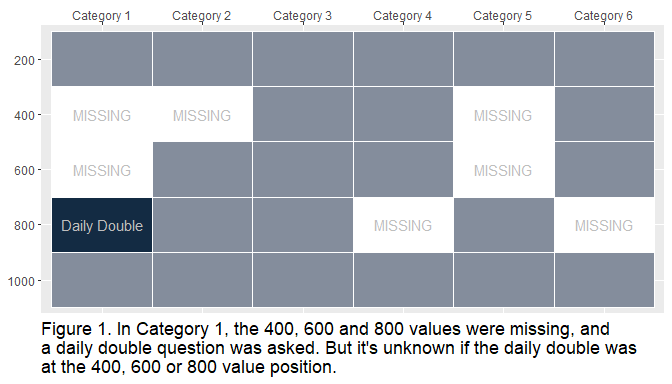
\includegraphics{final_presentation_files/figure-beamer/unnamed-chunk-2-1.pdf}

\end{frame}

\begin{frame}{Methods}
\protect\hypertarget{methods-2}{}

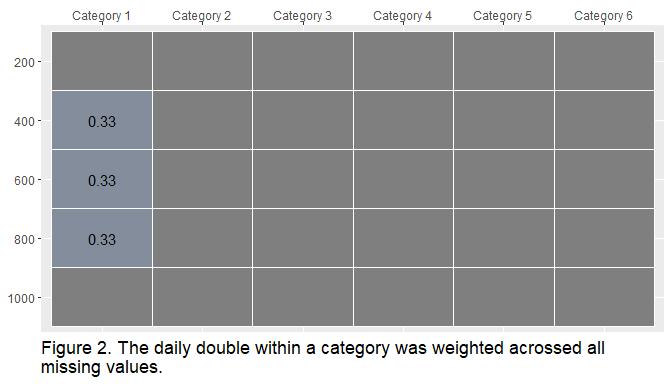
\includegraphics{final_presentation_files/figure-beamer/unnamed-chunk-3-1.pdf}

\end{frame}

\begin{frame}{Results}
\protect\hypertarget{results}{}

Flex Dashboard:

\begin{itemize}
\tightlist
\item
  Daily Double Round 1 since 2001
\item
  Daily Double Round 2 since 2001
\item
  Daily Double Location by year 
\item
  Daily Doubles are not evenly distributed across the board
\item
  No differences in daily double location between Round 1 and Round 2
\item
  15 out of 19 years had daily doubles within the 800/1600 row
\end{itemize}

\end{frame}

\begin{frame}{Conclusions}
\protect\hypertarget{conclusions}{}

\begin{itemize}
\tightlist
\item
  Similar to previous analyses

  \begin{itemize}
  \tightlist
  \item
    \url{https://flowingdata.com/2015/03/03/where-to-find-jeopardy-daily-doubles/}
  \end{itemize}
\item
  Shift in location in 2016

  \begin{itemize}
  \tightlist
  \item
    Arthur Chu and subsequent analyses 
  \end{itemize}
\item
  Future locations (pattern or random)
\end{itemize}

\end{frame}

\begin{frame}{Overview of Approach}
\protect\hypertarget{overview-of-approach}{}

Nest data by air date

Pull out subsets of that data

Modify subsets by:

Adding additional information (i.e.~weight, x/y position)

Manipulating data (i.e.~expanding, further subsetting)

Rejoin dataframes to get desired information

Create tidy dataset for plots

\end{frame}

\begin{frame}[fragile]{Interesting Packages or Techniques}
\protect\hypertarget{interesting-packages-or-techniques}{}

\begin{itemize}
\tightlist
\item
  Creating perfect data frame

  \begin{itemize}
  \tightlist
  \item
    Package: \texttt{tidyr}
  \item
    Function(s): \texttt{expand()} 
  \end{itemize}
\item
  Mapping

  \begin{itemize}
  \tightlist
  \item
    Package: \texttt{purrr}
  \item
    Function(s): \texttt{map()}, \texttt{map2()} 
  \end{itemize}
\item
  Joining

  \begin{itemize}
  \tightlist
  \item
    Package: \texttt{dplyr}
  \item
    Function(s): \texttt{right\_join()}, \texttt{full\_join()},
    \texttt{left\_join()} 
  \end{itemize}
\item
  Plotting

  \begin{itemize}
  \tightlist
  \item
    Package: \texttt{plotly}
  \item
    Function(s): \texttt{plot\_ly()}
  \end{itemize}
\end{itemize}

\end{frame}

\begin{frame}[fragile]{Examples}
\protect\hypertarget{examples}{}

\begin{itemize}
\tightlist
\item
  Input

  \begin{itemize}
  \tightlist
  \item
    \texttt{categories\_unique}: categories asked in each episode
  \item
    \texttt{categories\_asked}: information about asked questions
  \end{itemize}
\end{itemize}

\begin{Shaded}
\begin{Highlighting}[]
\KeywordTok{mutate}\NormalTok{(}\DataTypeTok{categories_unique =} \KeywordTok{map}\NormalTok{(categories_unique, }
                            \OperatorTok{~}\StringTok{ }\KeywordTok{rownames_to_column}\NormalTok{(., }\DataTypeTok{var =} \StringTok{"x_pos"}\NormalTok{)),}
         \DataTypeTok{perfect_pos =} \KeywordTok{map2}\NormalTok{(categories_unique, categories_asked, }
                            \OperatorTok{~}\StringTok{ }\KeywordTok{full_join}\NormalTok{(.x, .y)),}
         \DataTypeTok{perfect_pos =} \KeywordTok{map}\NormalTok{(perfect_pos, }
                           \OperatorTok{~}\StringTok{ }\KeywordTok{group_by}\NormalTok{(., round)),}
         \DataTypeTok{perfect_pos =} \KeywordTok{map}\NormalTok{(perfect_pos, }
                           \OperatorTok{~}\StringTok{ }\KeywordTok{expand}\NormalTok{(., x_pos, value)))}
\end{Highlighting}
\end{Shaded}

\begin{itemize}
\tightlist
\item
  Output

  \begin{itemize}
  \tightlist
  \item
    \texttt{categories\_unique}: x position assigned to each category
  \item
    \texttt{perfect\_pos}: perfect df for each game
  \end{itemize}
\end{itemize}

\end{frame}

\begin{frame}[fragile]{Examples}
\protect\hypertarget{examples-1}{}

\begin{itemize}
\tightlist
\item
  Input

  \begin{itemize}
  \tightlist
  \item
    \texttt{dd\_perfect}: perfect DD df
  \item
    \texttt{dd\_weight}: df containing the weight to be assiged to DD
    questions
  \end{itemize}
\end{itemize}

\begin{Shaded}
\begin{Highlighting}[]
\KeywordTok{mutate}\NormalTok{(}\DataTypeTok{dd_perfect =} \KeywordTok{map2}\NormalTok{(dd_perfect, dd_weight,}
                \OperatorTok{~}\StringTok{ }\KeywordTok{full_join}\NormalTok{(.x, .y, }\DataTypeTok{by =} \StringTok{"category"}\NormalTok{)),}
\DataTypeTok{dd_perfect =} \KeywordTok{map}\NormalTok{(dd_perfect, }
                 \OperatorTok{~}\StringTok{ }\KeywordTok{mutate}\NormalTok{(., }\DataTypeTok{daily_double =} \KeywordTok{case_when}\NormalTok{(}
                   \KeywordTok{is.na}\NormalTok{(daily_double) }\OperatorTok{==}\StringTok{ }\OtherTok{TRUE} \OperatorTok{~}\StringTok{ }\NormalTok{weight,}
                   \KeywordTok{is.na}\NormalTok{(daily_double) }\OperatorTok{==}\StringTok{ }\OtherTok{FALSE} \OperatorTok{~}\StringTok{ }\NormalTok{daily_double))))}
\end{Highlighting}
\end{Shaded}

\begin{itemize}
\tightlist
\item
  Output

  \begin{itemize}
  \tightlist
  \item
    \texttt{dd\_perfect}: perfect DD df with weights added
  \end{itemize}
\end{itemize}

\end{frame}

\begin{frame}[fragile]{Examples}
\protect\hypertarget{examples-2}{}

\begin{Shaded}
\begin{Highlighting}[]
\NormalTok{daily_double_year }\OperatorTok\StringTok{ }
\StringTok{  }\KeywordTok{unnest}\NormalTok{() }\OperatorTok\StringTok{ }
\StringTok{  }\KeywordTok{plot_ly}\NormalTok{(}
    \DataTypeTok{x =} \OperatorTok{~}\StringTok{ }\NormalTok{x_pos,}
    \DataTypeTok{y =} \OperatorTok{~}\StringTok{ }\NormalTok{y_pos,}
    \DataTypeTok{z =} \OperatorTok{~}\StringTok{ }\NormalTok{Percent,}
    \DataTypeTok{frame =} \OperatorTok{~}\StringTok{ }\NormalTok{year,}
    \DataTypeTok{hovertemplate =} \KeywordTok{paste}\NormalTok{(}\StringTok{"Daily Double Percent: %\{z:,\}%<br>"}\NormalTok{,}
                          \StringTok{"<extra></extra>"}\NormalTok{),}
    \DataTypeTok{colors =} \StringTok{"Blues"}\NormalTok{,}
    \DataTypeTok{type =} \StringTok{'heatmap'}
\NormalTok{) }\OperatorTok\StringTok{ }
\StringTok{  }\KeywordTok{layout}\NormalTok{(}\DataTypeTok{title =} \KeywordTok{list}\NormalTok{(}\DataTypeTok{text =} \StringTok{""}\NormalTok{), }
         \DataTypeTok{xaxis =} \KeywordTok{list}\NormalTok{(}\DataTypeTok{title =} \StringTok{""}\NormalTok{, }
                      \DataTypeTok{side =} \StringTok{'top'}\NormalTok{),}
          \DataTypeTok{yaxis =} \KeywordTok{list}\NormalTok{(}\DataTypeTok{title =} \StringTok{""}\NormalTok{))}
\end{Highlighting}
\end{Shaded}

\end{frame}

\begin{frame}[fragile]{Lessons Learned}
\protect\hypertarget{lessons-learned}{}

\begin{enumerate}
\tightlist
\item
  Seemingly simple problems may not be simple to answer.
\item
  Pros/cons of \texttt{ggplot} versus \texttt{plot\_ly}
\end{enumerate}

\end{frame}

\end{document}
